\documentclass[11pt]{article}

% Packages for professional formatting
\usepackage[margin=1in]{geometry}
\usepackage{times}
\usepackage[T1]{fontenc}
\usepackage[utf8]{inputenc}
\usepackage{microtype}
\usepackage{amsmath}
\usepackage{amssymb}
\usepackage{graphicx}
\usepackage{booktabs}
\usepackage{xcolor}
\usepackage{hyperref}
\usepackage{fancyhdr}
\usepackage{titlesec}
\usepackage{enumitem}
\usepackage{hyperref}
\usepackage{subcaption}
\usepackage{tikz}
\usetikzlibrary{arrows.meta, positioning, calc}

% Custom colors
\definecolor{mitred}{RGB}{163, 31, 52}
\definecolor{neuroblue}{RGB}{0, 82, 147}
\definecolor{darkgray}{RGB}{64, 64, 64}

\definecolor{summarygreen}{RGB}{34, 139, 34}     % Forest green - professional, readable
\definecolor{summarygray}{RGB}{105, 105, 105}   % Dim gray - subtle but visible  
\definecolor{summarynavy}{RGB}{25, 25, 112}     % Midnight blue - complements neuroblue
\definecolor{summarymaroon}{RGB}{128, 0, 0}     % Dark red - works with MIT theme

% Header and footer
\pagestyle{fancy}
\fancyhf{}
\lhead{\small BMIF 204 - Biomedical Informatics}
\rhead{\small Fall 2025}
\cfoot{\thepage}
\renewcommand{\headrulewidth}{0.4pt}

% Title formatting
\titleformat{\section}
{\color{neuroblue}\normalfont\Large\bfseries}
{\thesection}{1em}{}

\titleformat{\subsection}
{\color{darkgray}\normalfont\large\bfseries}
{\thesubsection}{1em}{}

\titlespacing*{\paragraph}
  {0pt}    % left indent
  {0.5ex}  % vertical space *before* the paragraph heading
  {1em}    % space between heading and text

% Hyperlink setup
\hypersetup{
    colorlinks=true,
    linkcolor=neuroblue,
    urlcolor=neuroblue,
    citecolor=neuroblue
}

% Single spacing
\linespread{1.0}
\setlength{\parskip}{0.5em}   % vertical space between paragraphs
\setlength{\parindent}{0pt}   % no indent at start of paragraphs

\bibliographystyle{ieeetr}

\begin{document}

% Title Page
\begin{center}
    {\LARGE \textbf{\color{mitred}Predicting Near-Term Adverse Drug Events in Polypharmacy: An Opioid-Focused Claims-Based Study}}\\[0.5cm]
    
    \rule{\linewidth}{0.5mm}\\[0.4cm]
    
    {\large 
    Benet Fité Abril, Yunxi Li, Ankit Pal
    }\\[0.3cm]
    
    \rule{\linewidth}{0.5mm}
\end{center}

\section{Abstract}


This study presents a scalable pipeline for transforming administrative claims data into a format suitable for identifying polypharmacy-related adverse drug events (ADEs) and evaluating their short-term predictability. Using Inovalon’s enterprise claims database, we constructed longitudinal “polypharmacy spells” and defined Time 0 as the moment a medication was added to a regimen of three or more concurrent drugs. For a focused use case, we analyzed opioid-involved spells due to their high clinical relevance \cite{liu_variation_2023}. The final cohort contained more than 800,000 spells from \~200,000 patients.

Despite substantial class imbalance (1.3\% ADE rate), machine learning models captured meaningful clinical signal. XGBoost modestly outperformed logistic regression (AUC-PR 0.0518 vs. 0.0441) and achieved a 15-fold enrichment of ADEs among the highest-risk predictions, though performance remained below clinical utility thresholds. Explainability analyses showed the models primarily detected markers of patient complexity rather than opioid-specific interactions. However, statistical tests identified several drug combinations with significantly elevated ADE incidence, including known opioid interaction partners.

This work establishes a reproducible pipeline for large-scale polypharmacy analysis and demonstrates the feasibility of near-term ADE risk prediction from claims data, while highlighting the need for expanded cohorts and richer clinical context to achieve deployable models.

\textit{DISCLAIMER: ChatGPT \cite{chatgpt} was used throughout this project as a coding assistant and literature researcher. In this report, no Generative AI is replacing our own intellectual effort, ChatGPT has only been used for rewriting, polishing and condensing information.}

\section{Introduction}

Polypharmacy, the concurrent use of multiple medications, is increasingly common in modern medicine and has been associated with elevated risk of adverse drug events (ADEs) \cite{komagamine_prevalence_2024}\cite{wang_prevalence_2024}. Although prior work has characterized the burden of polypharmacy and documented ADE frequency, far less is known about how specific drug combinations, patient characteristics, and regimen changes contribute to short-term ADE risk, particularly when medication regimens are modified. Understanding these interactions could enable clinicians to mitigate harm by identifying high-risk prescribing patterns at the point of medication change, supporting integration into electronic health record (EHR) decision support systems.

The objective of this study is (1) to develop a reusable data processing pipeline, (2) explore clinical and pharmacological factors associated with near-term ADEs following drug combination changes, and (3) evaluate whether machine learning models can predict these events from large-scale claims data. To ground the investigation in a clinically meaningful setting, we selected polypharmacy patients taking opioids, due to their high prevalence in the US and high rate of ADEs \cite{liu_variation_2023}.


\section{Methods}

\paragraph{\color{neuroblue}Eligibility Criteria:}
At the beginning of the project, our aim was too broad, as we intended to focus on all elderly polypharmacy patients. This yielded a very sparse cohort, so based on the preliminary results we decided to change the scope to members with $\geq$180 days of continuous pre-index enrollment (to balance comorbidity capture and cohort size), with $\geq$3 concurrent drugs including \textbf{at least one opioid} and without previous history of ADEs to avoid confounding. We removed the age restriction due to fewer than expected elderly patients in the cohort.

\paragraph{\color{neuroblue}Time Zero Definition:}
Due to the trends observed (see Results), which showed that many ADEs were occurring concurrently with drug additions to a patient’s prescription, we defined Time 0 as each time a patient added a drug to their combination, as long as the eligibility criteria were still met. The prediction target was defined as the occurrence of a new ADE within 30 days of this event.

\paragraph{\color{neuroblue}Data Source and Extraction:}
We used 1M and 5M patient samples from the Inovalon enterprise claims ecosystem, comprising prescription fills, inpatient/outpatient claims, ICD-10 diagnoses, demographics, and enrollment periods. ADE ICD-10 codes were curated from previous research \cite{hohl_icd-10_2014} identifying the codes more associated with ADEs, prioritizing classes A1, A2, B1, B2, and C. The selected list can be found \href{https://github.com/beni-1414/bmif204_claims_project/blob/main/data}{here}. For the selection of opioid drugs, National Drug Codes (NDC11) were downloaded from OpenFDA \cite{openfda}, filtered to opioid ingredients and normalized through ndclib-based conversions \cite{cosma_ndclib_2025}. The selected list can be found \href{https://github.com/beni-1414/bmif204_claims_project/blob/main/data}{here}.

The final pipeline extracts raw data from SQL servers filtering members based on the eligibility criteria, enables selective drug and ADE identification, and stores the data in parquet files in the O2 cluster. Due to traffic in the SQL database, we decided to offload as much processing as possible to O2 and python, avoiding the SQL bottleneck.

Before building the polypharmacy spells, drugs were clustered at the ATC3 class level to avoid artificially distinct representations of dose forms. NDC11 codes were first mapped to RxNorm using NDC-RxNorm crosswalk tool, then mapped to ATC3 using the sagerx tool \cite{nlm_rxnorm_crosswalk, coderxio_sagerx}. Comorbidities were clustered at the highest ICD-10 level (eg. A00).

\paragraph{\color{neuroblue}Spell Construction:}
After the raw data is downloaded into the cluster, a series of pandas-based python scripts build the polypharmacy spells using concurrent drug intervals, merging consecutive same-drug intervals, enforcing the eligibility criteria and allowing a grace period once counts drop below the minimum concurrent drugs, to account for prescription renewal delays. Since we were not working with time-to-event endpoints, we decided to set a minimum spell duration to remove short non-informative spells. In Figure \ref{fig:spell_building} the polypharmacy spell generation process is represented. Afterwards, the spells are split by drug additions to get our final time 0 aligned cohort and data cleaning is performed to maximize quality and avoid data leakage.

The detailed instructions to run the pipeline can be found \href{https://github.com/beni-1414/bmif204_claims_project/blob/main/README.md}{here}, with detailed information on the output tables. For the opioid use case, we chose a grace period of 15 days and a minimum spell duration of 15 days.

\paragraph{\color{neuroblue}Computational challenges:}
Due to the large size of the dataset, the code had to be optimized for performance, chunking, parallelizing and avoiding loading large tables into memory where possible. It is now possible to run the whole pipeline in around 10 hours on the 5M database, depending on SQL traffic. To scale to the full Inovalon dataset, the processing strategy would need to be refined.

Another challenge was ensuring the final tables were actually representing what was intended. Many data quality issues and bugs were identified in downstream EDAs and modeling results and subsequently corrected, yielding a pipeline robust to data leakage.

\paragraph{\color{neuroblue}Modeling Approaches:}
The objectives of the modeling were twofold: (1) to identify opioid drug combinations that are more strongly associated with ADE than baseline, and (2) to evaluate whether the incidence of ADE can be predicted within 30 days of a medication change. Our data set simulates a clinically actionable setting, where a predictive model could be triggered at the moment a new drug is added to a regimen, aligned with our Time 0 definition. 

To identify drug combinations with a significantly higher risk of ADE than average, we used \textbf{pairwise adjusted BH chi-square proportion tests}. It does not correct for comorbidity confounders, but can provide interesting directions for future in-depth causal studies on the full Inovalon dataset.

For prediction, both classical ML and DL methods were explored. The predictors used were comorbidities, drugs on prescription, age, gender and race.  For ML, multi-hot encoding was used for drugs and comorbidities, and one-hot encoding was used for demographics. The approaches explored in this study are:
\begin{itemize}
    \item \textbf{Baseline logistic regression}: interpretable and baseline predictive benchmark, allows for identification of high odds-ratio factors with confounder adjustment. To account for imbalance, we used l2 regularization, the saga solver and a class-weighted loss function.
    \item \textbf{XGBoost}: gradient-boosted trees with strong performance in sparse tabular datasets, which allows for the use of SHAP to identify the weight of specific variables on decision trees. To account for imbalance, we optimized the parameter scale\_pos\_weight to $0.2*ADE prevalence$.
    \item \textbf{Multilayer Perceptron + MedTok}: a basic but powerful DL model that allowed us to try MedTok \cite{su_multimodal_2025-1}, a library that provides pretrained embeddings for the ATC classes and ICD comorbidities based on a knowledge graph. Multiple architectures for the embeddings (flatten, mean, attention) and various hidden layer sizes were explored.
\end{itemize}

For the evaluation, we opted for:
\begin{itemize}
    \item \textbf{AUC-PR} - The primary performance metric due to the very low prevalence of events, as it focuses on how well the model identifies the minority class. Interpreting AUC-PR relative to the ADE prevalence allows us to quantify how much better than random guessing the model is performing.
    \item \textbf{AUC-ROC} - Included as a secondary metric, although it is not optimal for highly imbalanced datasets.
    \item \textbf{Precision@k}: to see the ability of the models to rank positive cases higher than negative ones.
    \item \textbf{Recall@x precision}: to put the real-world impact of the predictive algorithms in easily understandable terms: \textit{if I want a precision of x\%, what will my recall be?}
\end{itemize}

\paragraph{\color{neuroblue}Generalizability of method:}
The polypharmacy analysis pipeline developed here is adaptable to a wide range of research objectives. It can support broad investigations such as the opioid-focused use case explored in this study, or highly targeted analyses of specific drug combinations or ADE types. Its modular structure facilitates extension, and further engineering work could enable deployment across Inovalon’s 200M claims database.

\section{Results}
\paragraph{\color{neuroblue}Cohort Overview:}
The final cohort represented in the CONSORT diagram in Figure \ref{fig:CONSORT_claims} included 814,412 opioid-involved polypharmacy spells from 206,664 patients, of which 10,898 (1.3\%) suffered an ADE within 30 days of a drug change. Demographic and medication-pattern distributions, including age, gender, race and comorbidity counts, were consistent with expectations for a high-utilization population (Table \ref{tab:spell_baseline}), indicating no systematic biases in cohort construction.

Analysis of ADE patterns revealed a pronounced temporal signal: after aligning spells by Time 0, there was a significant data shift: \~80\% of ADEs occurred within 30 days of the regimen change, and most were opioid- or dosage-related (Figure \ref{fig:claims_ADE_distribution}), vs only \~35\% in the non-splitted data. This concentration of clinically coherent events immediately following medication adjustments supports the relevance of our outcome definition and motivates the use of predictive models targeting near-term ADE risk.

In the annex you can find lists with the drug combinations associated with a higher ADE prevalence, with the relevant chi-sq p-value compared against the rest of the cohort (Table \ref{tab:drug_pairs_ae_min200_with_BH}, \ref{tab:drug_trios_ae_min200_with_BH}).

\paragraph{\color{neuroblue}Model Performance and interpretability:}
With a baseline risk for a 30-day ADE of 1.3\%, this was a challenging prediction task. Logistic regression modestly exceeded this baseline, achieving an AUC-PR of 0.0441 and concentrating 16.0\% ADE prevalence in the top 0.1\% of alerts. XGBoost delivered the strongest performance, increasing AUC-PR to 0.0518 and achieving 20.3\% precision in the top 0.1\% of predictions, a 15x enrichment over baseline (Figure \ref{tab:model_performance}). The neural MLP-MedTok approach underperformed the tree-based model, and would require more architectural tuning and probably more data to ensure enough signal.

Feature attribution analyses using odds ratios (logistic regression) and SHAP values (XGBoost) revealed distinct clinical and pharmacological drivers of model predictions (Figures \ref{fig:odds_ratios_logreg}, \ref{fig:xgboost_interpret}), which are explored in greater detail in the Discussion.

\section{Discussion}
First of all, the analysis of the opioid cohort and the interpretability metrics of the models allowed us to validate the robustness and correctness of the pipeline. Proportion-based test results were consistent with reported drug-drug interactions \cite{feng_opioid_2017}: antiemetics (A04A) have been reported to cause enhanced opioid exposure and sedation, and antipsychotics (N05A) have been reported by the FDA to have risk of synergistic respiratory depression and risk of overdose \cite{szmulewicz_risk_2021}. Most other high p-value pairs, for example chemotherapy agents (L01X/L01E/L01A), likely reflect complex pharmacokinetic interactions, contextual acuity (ICU stays) and general patient frailty, rather than specific interaction with opioids.

Although the predictive performance of our models remains modest by clinical standards, the observed enrichment at the high end of the risk spectrum indicates that adverse drug events are not randomly distributed in this population and that the database contains some genuine pharmacologic and clinical signal, even though the performance is far from a clinically deployable model.

Some limitations that could explain the low performance come from claims data itself and from the study design. Regarding claims data, the main issue is that it lacks dosage timing, so so we made a general assumption of one dose per day. This could be improved in studies with a narrower set of drugs by curating a table of dosage / drug. Also, as it is common in pharmacy fills, you never know if the patient actually took the prescription or not. The dataset also does not capture non-prescription drugs such as NSAIDs, which could interact with other drugs and confound results.

Regarding the study design, there are two main limitations: clustering and cohort size. For drugs, we are clustering at the ATC3 level, as we are covering a broad range of drugs and allowed to identify general associations. Ideally a more narrow clinical question should cluster at more granular levels, to avoid loss of information. For comorbidities, we are clustering ICD codes to the highest level of the tree. More complex approaches such as PheCodes \cite{wu_mapping_2019} or other clinically meaningful comorbidity scores should be explored in future studies. With respect to the cohort size, scaling to the 200M dataset would allow deep learning approaches, leveraging MedTok to encode the drugs and comorbidities in a meaningful way as we showed in our proof of concept. The pre-index window could also be extended, even if at risk of adding noise to the models.

The interpretability plots provide a final layer of insight towards the interpretation of the results. Both logistic regression and XGBoost mostly focus on drugs and comorbidities that act as proxies of general patient complexity and general ADE predictors, rather than specific opioid related interactions or factors. This suggests that predicting ADEs within an opioid-focused polypharmacy cohort may not have been the optimal design choice, and suggests two possible directions for improving prediction are:
\begin{itemize}
    \item Go back to our initial hypothesis and try to generally capture the indicators of patient complexity and frailty on a general dataset of polypharmacy, allowing a big deep learning model to cluster and separate the patients based on their comorbidities and drug prescriptions. This approach however risks predicting that \textit{sicker patients get more ADEs}, which is not that clinically useful.
    \item Narrow down the definition of what opioid patient profile we are focusing on (chronic pain vs cancer patients vs addictive disorders, etc) and develop more homogeneous class-specific models, to see if the predictions improve on the stratified groups.
\end{itemize}

\paragraph{\color{neuroblue}Learnings and personal reflection:}
This project allowed us to battle with the complexities of claims data, exposing the temporal power of this kind of data and its shortcomings. It also taught us that having a clear clinical question is very important to be able to produce meaningful results, as a common struggle during the semester was the lack of specificity of the clinical question and the constant refining of it. %If I have time, I will reuse the pipeline to try to answer a narrower clinical question, emulating some of the fantastic methods my classmates have used.

\paragraph{\color{neuroblue}Next steps:}
Apart from the two possible study design variations described in the discussion, this project's insights point towards an interesting series of next steps:
\begin{itemize}
    \item \textbf{Scale up}: adapt the code to work on the 200M database, leveraging SQL and the O2 resources efficiently.
    \item \textbf{Pharmacoepidemiology drug-drug interactions}: more interesting than predicting that sicker patients get more ADEs, the pipeline could be reused to do sensitivity analysis on drug combinations, using specific ADE occurrence as an endpoint. One example of question that could be answered with small tweaks to the pipeline is: Among adults with chronic non-cancer pain already receiving long-term opioid therapy, what is the effect of initiating gabapentin vs initiating duloxetine as an adjunct analgesic on the risk of serious opioid-related adverse drug events (overdose, respiratory depression, ED visit, hospitalization)? \cite{hahn_risk_2022,gomes_gabapentin_2017}
    \item \textbf{Merging with EHR}: A model predicting ADEs would be deployed in an EHR, so maybe leveraging the increased information density of the EHR would yield better results.
    \item \textbf{Automation}: Claims data is very difficult to work with, both due to the format of the data itself and the size of it. User-friendly AI wrapping of the pipeline could allow professionals with less computational knowledge to run preliminary cohort size assessment and exploration, and even run simple end-to-end analysis.
\end{itemize}


\bibliography{Claims_project/references}

\section{Acknowledgements}
We would like to thank Inovalon for allowing us access to their datasets. All work was performed as part of Harvard's BMIF204 course, taught by Sebastian Schneeweiss.

\section{Reproducibility}
Code is available at \url{https://github.com/beni-1414/bmif204_claims_project}.

\appendix
\section{Figures and tables}

\begin{figure}[htbp]
    \centering
    \includegraphics[width=0.8\linewidth]{Claims_project/figures/spell_generation.png}
    \caption{Representation of the spell building timeline for a patient. The parameters involved are window length, grace period, minimum concurrent drugs and minimum spell length, as well as the list of ICD-10 ADEs and target NDC drugs.}
    \label{fig:spell_building}
\end{figure}

\begin{figure}[htbp]
    \centering
    % consort_diagram.tex
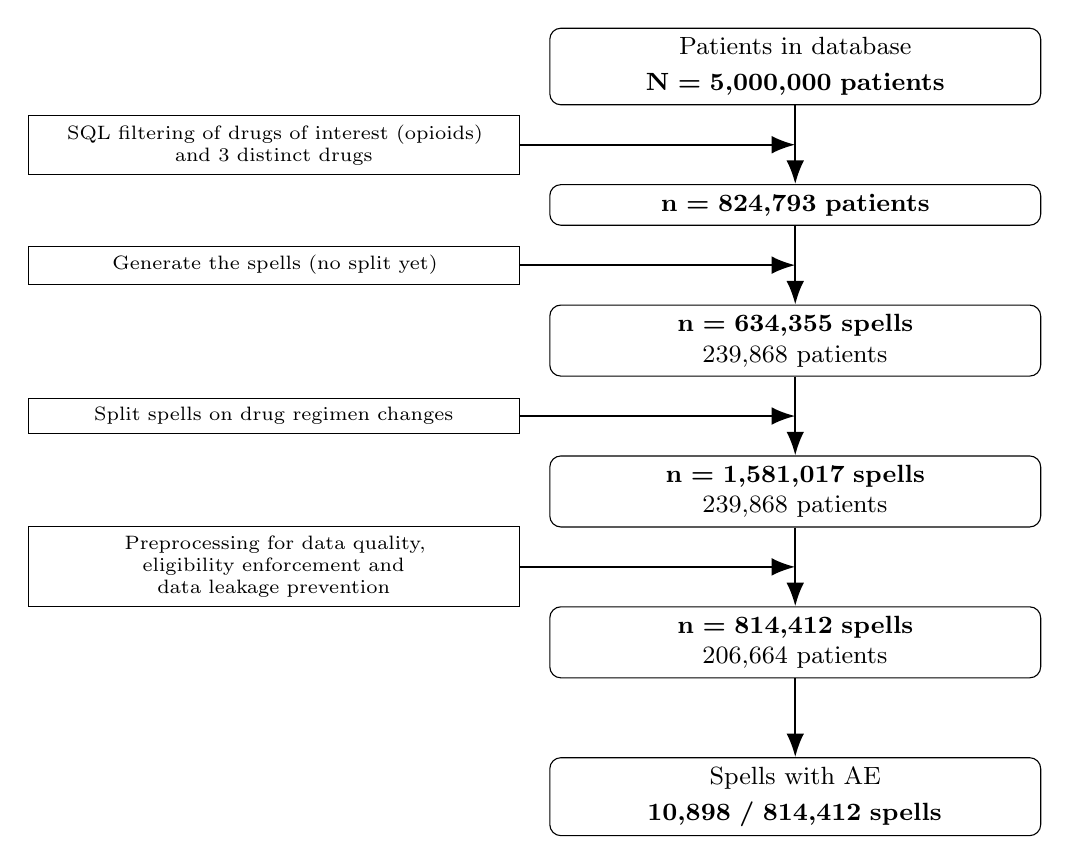
\begin{tikzpicture}[
  node distance=10mm,
  cohort/.style={
    rectangle,
    draw,
    rounded corners,
    align=center,
    font=\small,
    text width=6cm,
  },
  filter/.style={
    rectangle,
    draw,
    align=center,
    font=\scriptsize,
    text width=6cm,
  },
  arrow/.style={-{Latex[length=3mm]}, thick}
]

% ===== VERTICAL COHORT NODES (ONLY SIZES) =====
\node[cohort] (p0) {Patients in database\\[2pt]
  \textbf{N = 5,000,000 patients}
};

\node[cohort, below=of p0] (p1) {
  \textbf{n = 824,793 patients}
};

\node[cohort, below=of p1] (p2) {
  \textbf{n = 634,355 spells}\\
  239,868 patients
};

\node[cohort, below=of p2] (p3) {
  \textbf{n = 1,581,017 spells}\\
  239,868 patients
};

\node[cohort, below=of p3] (p4) {
  \textbf{n = 814,412 spells}\\
  206,664 patients
};

\node[cohort, below=of p4] (p5) {
  Spells with AE\\[2pt]
  \textbf{10,898 / 814,412 spells}
};

% ===== VERTICAL ARROWS =====
\draw[arrow] (p0) -- (p1);
\draw[arrow] (p1) -- (p2);
\draw[arrow] (p2) -- (p3);
\draw[arrow] (p3) -- (p4);
\draw[arrow] (p4) -- (p5);

% Convenience coordinates: midpoints of vertical segments
\coordinate (m1) at ($(p0.south)!0.5!(p1.north)$);
\coordinate (m2) at ($(p1.south)!0.5!(p2.north)$);
\coordinate (m3) at ($(p2.south)!0.5!(p3.north)$);
\coordinate (m4) at ($(p3.south)!0.5!(p4.north)$);

% ===== SIDEWAYS FILTER / ACTION ARROWS =====

% SQL filtering -> between p0 and p1
\node[filter, left=35mm of m1] (f1) {
  SQL filtering of drugs of interest (opioids)\\
  and 3 distinct drugs
};
\draw[arrow] (f1.east) -- (m1);

% Generate spells (no split) -> between p1 and p2
\node[filter, left=35mm of m2] (f2) {
  Generate the spells (no split yet)
};
\draw[arrow] (f2.east) -- (m2);

% Split spells -> between p2 and p3
\node[filter, left=35mm of m3] (f3) {
  Split spells on drug regimen changes
};
\draw[arrow] (f3.east) -- (m3);

% Preprocessing -> between p3 and p4
\node[filter, left=35mm of m4] (f4) {
  Preprocessing for data quality,\\
  eligibility enforcement and\\
  data leakage prevention
};
\draw[arrow] (f4.east) -- (m4);

\end{tikzpicture}

    \caption{CONSORT-style diagram of the data extraction and processing steps, starting from the 5M member Inovalon sample.}
    \label{fig:CONSORT_claims}
\end{figure}

\begin{table}[htbp]
    \centering
    \caption{Baseline characteristics of opioid spells with and without an adverse event (ADE) within 30 days.}
    \input{Claims_project/figures/table1}
    \label{tab:spell_baseline}
\end{table}

% The figure below should include the ADE timing plot and the top ADE names and frequencies. There is both the plot and the numerical info if a table feels better.
\begin{figure}[htbp]
    \centering
    
    % (a) Top ADE categories — also acts as legend
    \begin{subfigure}[b]{0.9\textwidth}
        \centering
        \includegraphics[width=\linewidth]{Claims_project/figures/ADE_distribution_plot.png}
        \caption{Top adverse event (ADE) categories, aggregated by ICD-10 description. 
        Bar colors match the timing distributions in panel (b).}
        \label{fig:ae_top_categories}
    \end{subfigure}
    
    \vspace{0.8em}
    
    % (b) ADE timing within spells
    \begin{subfigure}[b]{0.9\textwidth}
        \centering
        \includegraphics[width=\linewidth]{Claims_project/figures/ADE_timing_within_spell_5M.png}
        \caption{Timing of ADE occurrence within polypharmacy spells, comparing original and split spell definitions.}
        \label{fig:ae_timing_within_spell}
    \end{subfigure}
    
    \caption{Distribution and timing of adverse events (ADEs) in the opioid-involved polypharmacy cohort.}
    \label{fig:claims_ADE_distribution}
\end{figure}

\begin{table}[htbp]
    \centering
    \caption{Drug Pairs Ae Min200 With Bh (EDIT ME)}
    \label{tab:drug_pairs_ae_min200_with_BH}
\begin{tabular}{llrrrrrr}
\toprule
drug1 & drug2 & n\_total & n\_ae & n\_no\_ae & ae\_prop & p\_value & p\_adj \\
\midrule
B05B & N02A & 476 & 31 & 445 & 6.51e-02 & 1.12e-12 & 2.43e-11 \\
L01A & N02A & 209 & 13 & 196 & 6.22e-02 & 2.00e-05 & 1.49e-04 \\
L01E & N02A & 1428 & 87 & 1341 & 6.09e-02 & 6.03e-30 & 4.33e-28 \\
L01X & N02A & 1115 & 57 & 1058 & 5.11e-02 & 2.24e-14 & 5.59e-13 \\
L03A & N02A & 943 & 46 & 897 & 4.88e-02 & 9.16e-11 & 1.59e-09 \\
C01C & N02A & 2351 & 110 & 2241 & 4.68e-02 & 4.95e-22 & 2.16e-20 \\
H01B & N02A & 252 & 11 & 241 & 4.37e-02 & 9.65e-03 & 3.51e-02 \\
N01A & N02A & 899 & 38 & 861 & 4.23e-02 & 9.57e-07 & 9.17e-06 \\
N02A & V03A & 5247 & 218 & 5029 & 4.15e-02 & 8.73e-32 & 6.63e-30 \\
A07A & N02A & 3721 & 148 & 3573 & 3.98e-02 & 1.25e-19 & 4.67e-18 \\
A11D & N02A & 789 & 30 & 759 & 3.80e-02 & 2.10e-04 & 1.23e-03 \\
A04A & N02A & 35480 & 1289 & 34191 & 3.63e-02 & 3.45e-126 & 2.78e-123 \\
A12C & N02A & 400 & 14 & 386 & 3.50e-02 & 3.50e-02 & 1.03e-01 \\
A03F & N02A & 5221 & 181 & 5040 & 3.47e-02 & 6.79e-16 & 1.95e-14 \\
N02A & N04A & 1671 & 57 & 1614 & 3.41e-02 & 1.48e-05 & 1.13e-04 \\
A05A & N02A & 1038 & 34 & 1004 & 3.28e-02 & 2.27e-03 & 1.02e-02 \\
C01E & N02A & 1711 & 56 & 1655 & 3.27e-02 & 7.21e-05 & 4.76e-04 \\
A09A & N02A & 2206 & 72 & 2134 & 3.26e-02 & 6.81e-06 & 5.58e-05 \\
B03X & N02A & 401 & 13 & 388 & 3.24e-02 & 8.26e-02 & 2.06e-01 \\
N02A & N07B & 14793 & 478 & 14315 & 3.23e-02 & 3.12e-31 & 2.28e-29 \\
\bottomrule
\end{tabular}

\end{table}

\begin{table}[htbp]
    \centering
    \caption{Drug Trios Ae Min200 With Bh (EDIT ME)}
    \label{tab:drug_trios_ae_min200_with_BH}
\begin{tabular}{lllrrrrrr}
\toprule
drug1 & drug2 & drug3 & n\_total & n\_ae & n\_no\_ae & ae\_prop & p\_value & p\_adj \\
\midrule
C01C & H02A & N02A & 378 & 37 & 341 & 9.79e-02 & 7.70e-28 & 2.72e-25 \\
H02A & L01E & N02A & 201 & 19 & 182 & 9.45e-02 & 6.01e-14 & 4.92e-12 \\
A04A & M04A & N02A & 464 & 42 & 422 & 9.05e-02 & 3.76e-28 & 1.40e-25 \\
A04A & N02A & N05A & 2728 & 236 & 2492 & 8.65e-02 & 9.75e-144 & 2.07e-139 \\
A04A & N02A & V03A & 446 & 36 & 410 & 8.07e-02 & 1.81e-20 & 3.25e-18 \\
A04A & A09A & N02A & 314 & 25 & 289 & 7.96e-02 & 3.53e-14 & 3.04e-12 \\
A04A & L01E & N02A & 252 & 20 & 232 & 7.94e-02 & 1.90e-11 & 1.03e-09 \\
A07A & H02A & N02A & 560 & 44 & 516 & 7.86e-02 & 8.21e-24 & 1.95e-21 \\
A04A & C02A & N02A & 650 & 51 & 599 & 7.85e-02 & 2.16e-27 & 7.39e-25 \\
A07A & N01B & N02A & 232 & 18 & 214 & 7.76e-02 & 4.80e-10 & 2.09e-08 \\
B05X & N02A & V03A & 225 & 17 & 208 & 7.56e-02 & 3.60e-09 & 1.31e-07 \\
A04A & A07A & N02A & 467 & 35 & 432 & 7.49e-02 & 8.76e-18 & 1.06e-15 \\
A04A & N02A & N07B & 873 & 65 & 808 & 7.45e-02 & 7.23e-32 & 3.65e-29 \\
A04A & A07D & N02A & 616 & 44 & 572 & 7.14e-02 & 1.75e-20 & 3.16e-18 \\
C08D & J01E & N02A & 249 & 17 & 232 & 6.83e-02 & 6.77e-08 & 1.87e-06 \\
H03A & N02A & V03A & 371 & 25 & 346 & 6.74e-02 & 5.51e-11 & 2.85e-09 \\
A10A & N02A & P01A & 239 & 16 & 223 & 6.69e-02 & 2.92e-07 & 6.85e-06 \\
L01E & N02A & N02B & 284 & 19 & 265 & 6.69e-02 & 1.84e-08 & 5.79e-07 \\
C07A & L01E & N02A & 212 & 14 & 198 & 6.60e-02 & 2.53e-06 & 4.63e-05 \\
A03B & A04A & N02A & 276 & 18 & 258 & 6.52e-02 & 9.47e-08 & 2.51e-06 \\
\bottomrule
\end{tabular}

\end{table}


\begin{table}[ht]
\centering
\begin{tabular}{lcccc}
\hline
Methods & AUROC & AUPRC$^{*}$ & Precision @ top 0.1\% & Precision @ top 5\% \\
\hline
Logistic regression & 0.7441 & 0.0441 & 16.0\% & 5.8\% \\
XGBoost             & \textbf{0.7672} & \textbf{0.0518} & 20.3\% & 6.3\% \\
MLP + MedTok        & 0.7186 & 0.0381 & -- & -- \\
\hline
\end{tabular}
\caption{Model performance on ADE prediction (ADE rate \~1.3\%).}
\label{tab:model_performance}
\end{table}

\begin{figure}[htbp]
    \centering
    \includegraphics[width=0.8\linewidth]{Claims_project/figures/odds_ratios.png}
    \caption{Odds ratios from the LogReg baseline analysis. Drugs are in ATC3 codes. The CIs could be built with bootstrapping.}
    \label{fig:odds_ratios_logreg}
\end{figure}

\begin{figure}[htbp]
    \centering
    % SHAP summary plot (vertical image)
    \begin{subfigure}[b]{0.6\textwidth}
        \centering
        \includegraphics[width=\linewidth]{Claims_project/figures/SHAP_5M.png}
        \caption{SHAP summary plot of feature contributions for the XGBoost model.}
        \label{fig:shap_summary}
    \end{subfigure}
    \hfill
    % PR curve
    \begin{subfigure}[b]{0.48\textwidth}
        \centering
        \includegraphics[width=\linewidth]{Claims_project/figures/pr_curve.png}
        \caption{Precision–recall curve of the best-performing XGBoost model.}
        \label{fig:pr_curve}
    \end{subfigure}
    
    \caption{Interpretability and performance plots for XGBoost model.}
    \label{fig:xgboost_interpret}
\end{figure}

\end{document}